\section{Metrics and benchmarks}
Before running topic modelling, it is useful to define some metrics to test and benchmark the model. In particular the model search sets on the two sides of the network the one containing samples and the one containing genes. Samples are extracted from datasets where much metadata are available, some of these metadata labels will be used to benchmark the model. To study genes enrichment test are necessary.

Looking at the samples side of the network, the outputs are sets of samples, the clusters. One can state the model works if all, or at least the majority, of samples in the same cluster share some label. Here the tissue is considered as the main label.

Note that this work's model is a non supervised one, but a ground truth is available from metadata. So every sample has a certain probability to have a certain property (the true tissue label), let's call this $P(C)$ and a certain probability of being in a cluster (model's output), let's call this $P(K)$.
It is possible to define some quantities, the homogeneity
\begin{equation}\label{eq:homogeneity}
    h=1-\frac{H(C|K)}{H(C)}
\end{equation}
defining the entropy
\begin{equation}\label{eq:hck}
    H(C|K)=\sum_{c\in \mathrm{tissues},\\ k \in \mathrm{clusters}}\frac{n_{c k}}{N}Log\left(\frac{n_{c k}}{n_k}\right)
\end{equation}
where $n_{c k}$ is the number of nodes of type $c$ in cluster $k$, $N$ the number of nodes and $n_k$ the number of nodes in cluster $k$. It is evident that if all nodes inside cluster $k$ are of the same type $c$ $n_{c k}=n_{k}$, $H(C|K)=0$ and $h=1$, it is actually a complete homogeneous situation.

Another quantity can be defined and it is completeness:
\begin{equation}\label{eq:completness}
    c=1-\frac{H(K|C)}{H(K)},
\end{equation}
$H(K|C)$ is defined in the same way as~\ref{eq:hck}. Completeness measures how well nodes of the same type are distributed in the same cluster.

Ideally one wants a method which output is both homogeneous and complete. So it is possible to define the V-measure as the harmonic average of the two:
\begin{equation}\label{eq:mutualinformation}
    \mathrm{V-measure}=2\frac{h c}{h + c},
\end{equation}
which is actually the normalized mutual information between $P(C)$ and $P(K)$~\cite{rosenberg2007v}. Please refer to appendix~\ref{app:vmeasure} to the detailed math. In figure~\ref{fig:topic/metric_scores_primarysite} an example of the V-measure score estimated at the different layers of the hierarchy; note that the number of clusters increases going deeper in the hierarchy. In the same figure homogeneity and completeness are reported, note that with few clusters the situation is more complete, but when the number of clusters increases completeness goes down and homogeneity increase. 
\begin{figure}[htb!]
    \centering
    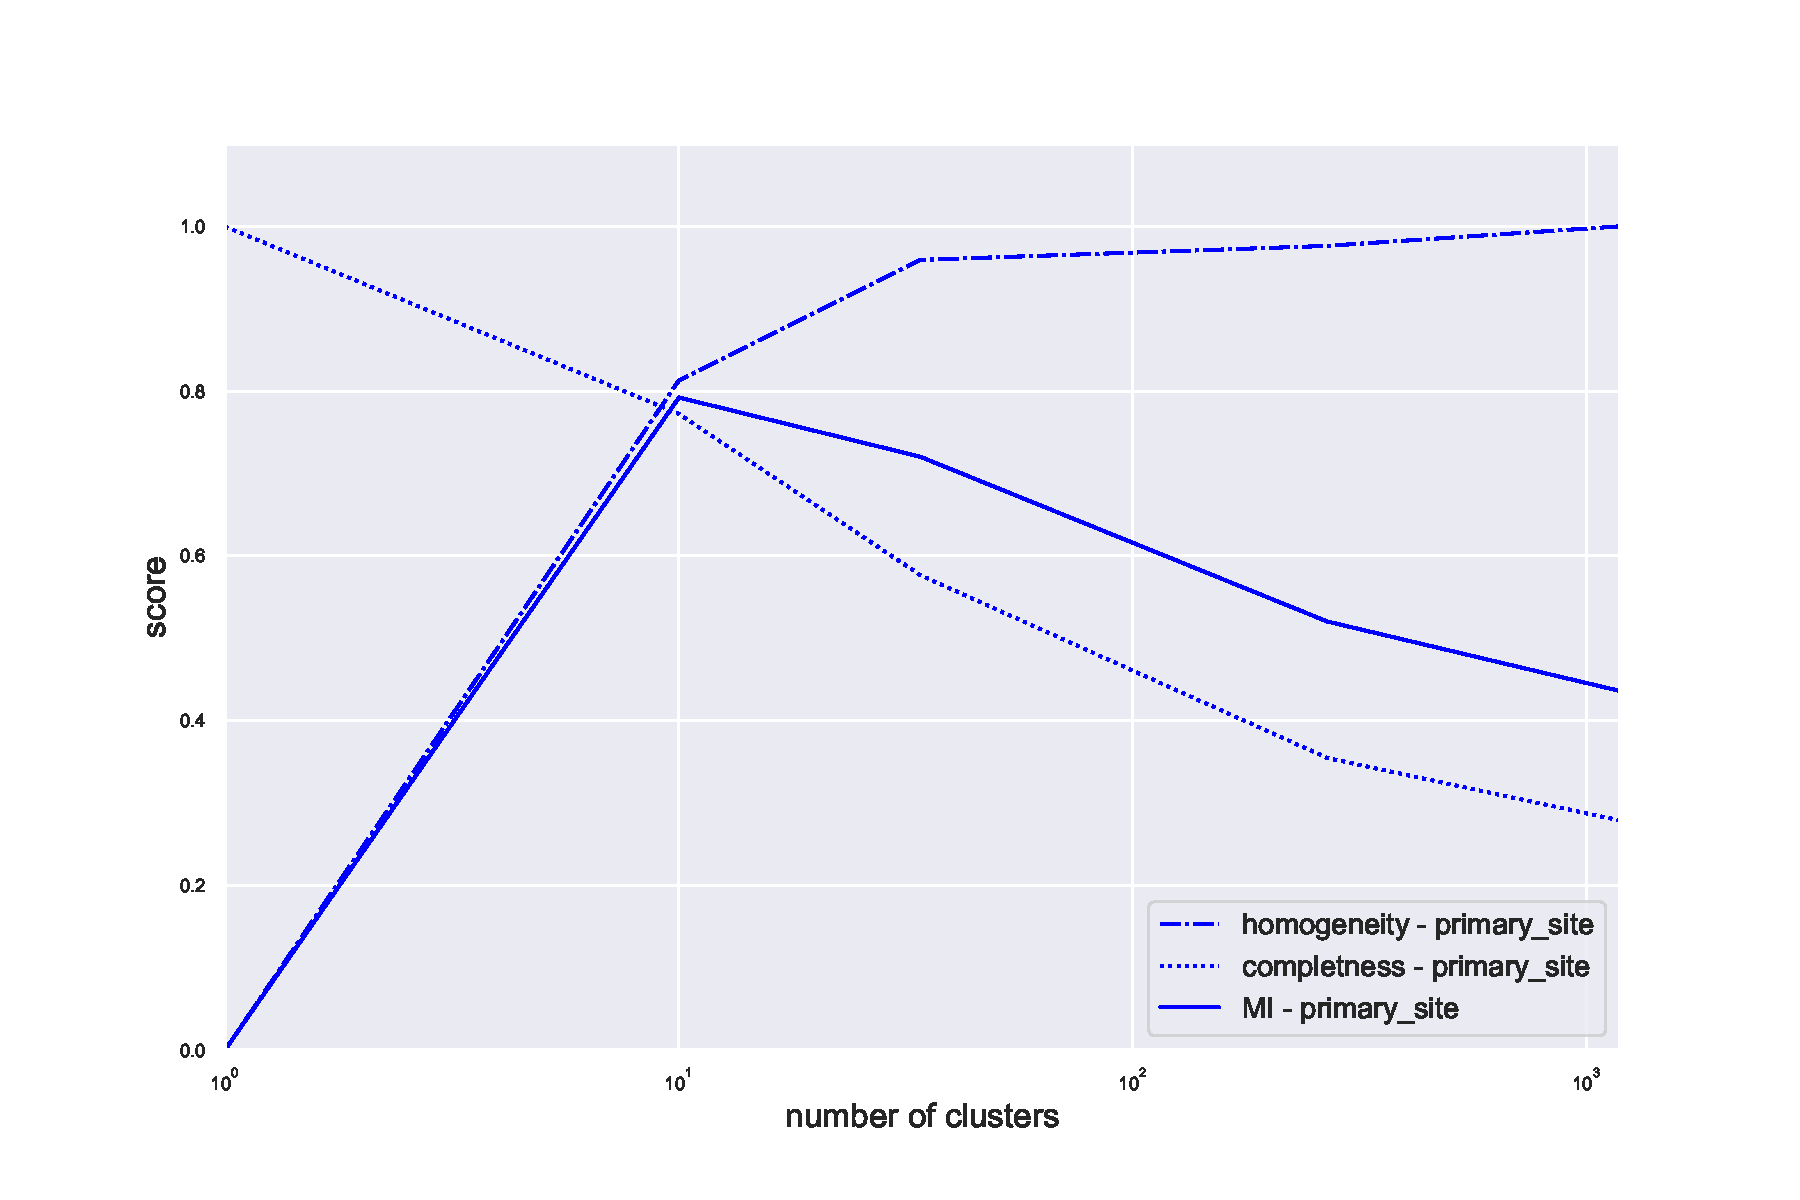
\includegraphics[width=0.9\linewidth]{pictures/topic/gtex/oversigma_10tissue/metric_scores_primarysite.pdf}
    \caption{Score across hierarchy. The V-measure or normalized mutual information MI is the harmonic average between homogeneity and completeness.}
    \label{fig:topic/metric_scores_primarysite}
\end{figure}

In the next sections will be studied also the maximum fraction of label in the same cluster defined as 
\[max_{c\in k}\frac{n_{c k}}{n_k}.\] Also the number of different labels in the same cluster will be studied.
\FloatBarrier